\chapter{Realisierung}
\label{chap:Realisierung}

Dieses Kapitel beschreibt die Realisierung des Prototyps. Der Prototyp ist eine überarbeitete Version der Konzeptvariante 2 , siehe \ref{sec:var2}. Es mussten Änderungen bei verschiedenen Komponenten durchgeführt werden, diese werden in den nachfolgenden Unterkapitel \ref{sec:mechKomp} erläutert. 


\section {Hardware}
\label{sec:Hardware}

Da beide Projekte, welche im Unterkapitel \ref{sec:Vorzeigeprojekte} eine endlos drehende Konstruktion nutzten, sowie die Aufgabenstellung im Anhang \ref{Pflchtenheft} eine drehende Konstruktion vorgibt, wurde eine endlos drehende mechanishce Konstruktion gewählt. 

\subsection {mechanische Komponenten \& Gehäuse}
\label{sec:mechKomp}


Um eine möglichst einfache und schnelle Lösung zu realisieren, wurden die mechanischen Komponenten nach Verfügbarkeit ausgewählt. Die Masse des Alurohrs und der Zahnräder waren größtenteils durch die Rösser des Kugellagers gegeben. Das Kugellager wurde so gewählt, dass ein Ethernet RJ45 Stecker hindurchgeführt werden kann, da der gewählte Schleifring ein vorkonfektionierten RJ45-Stecker besitzt.

Das Kugellager wurde direkt auf das Alurohr gepresst und zusätlich mit Schrauben verkeilt.

Die Zanhräder wurden mit dem Tool Onshape gelayoutet und im FabLaab mit einem 3D-Drucker erzeugt. Aus den vorgegebenen Dimensionen wurde ein Übersetzungsverhalnis der Zahnräder von 1.5 gewählt. 

Dabei wurden in einer ersten Version 

\begin{figure}[H]
	\centering
	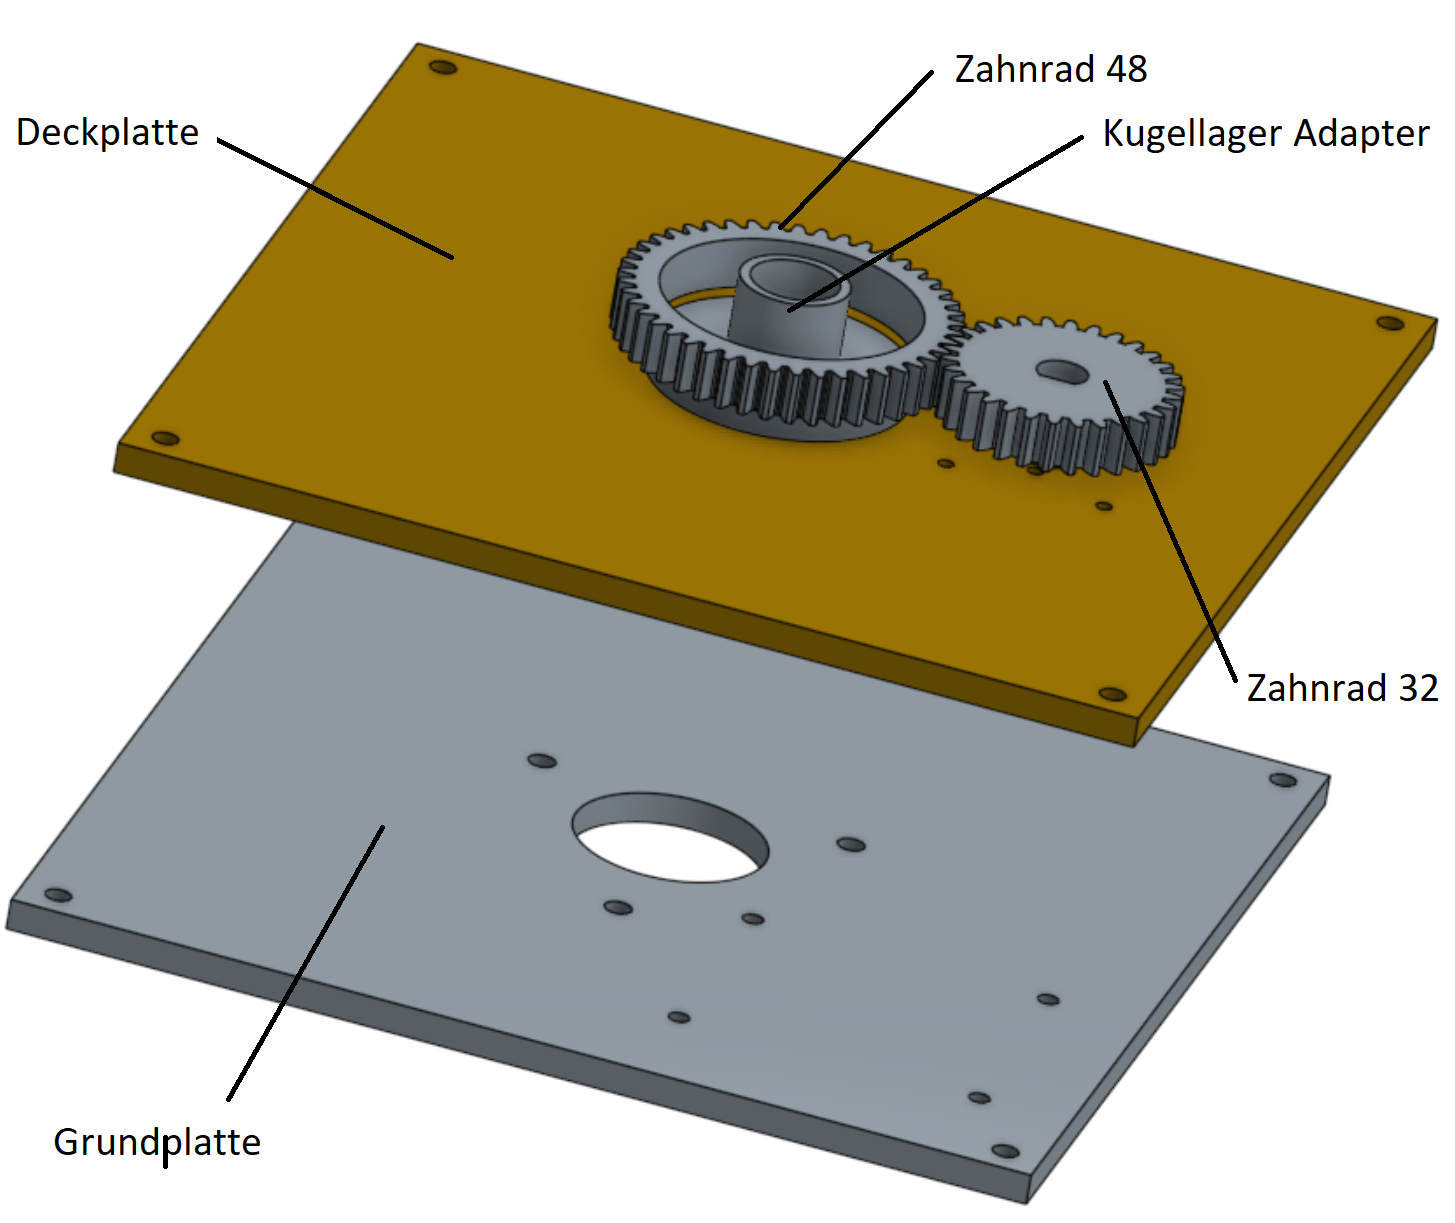
\includegraphics[width=0.8\textwidth]{resources/mechKomp2.PNG}
	\caption{zusammengefügte mechanische Komponenten}
	\label{fig:mechKomp}
\end{figure} 


Die Grösse der Platten wurde so gewählt, dass alle Komponenten dazwischen verbaut werden können. Daher wurden zwei MDF-Platten mit den Massen 200mm x 200mm x 6mm (HxBxT) im Fablab erstellt. Die Grund- und Topplatten wurden in OnShape gelayoutet un 
\subsection {elektrische Komponenten}
\label{sec:elekKomp}



% verkabelungsskizze

\section{Software}
\label{sec:SoftwareReal}

%  


\subsection {3D Mapping}
\label{sec:3DMapping}

\subsection {Motorenansteuerung}
\label{sec:Motorenansteuerung}

\section{Zwischenfazit}
\label{sec:ZwischenfazitReal}